\documentclass{article}

%other packages
\usepackage[a4paper]{geometry}
\usepackage{longtable}
\usepackage{wrapfig}
\setlength\parindent{0pt}
\usepackage{enumitem}
\usepackage[table,dvipsnames]{xcolor}
\usepackage{polynom}
\def\scaleint#1{\vcenter{\hbox{\scaleto[3ex]{\displaystyle\int}{#1}}}}
\usepackage{array}
\newcolumntype{C}{>{{}}c<{{}}} % for '+' and '-' symbols
\newcolumntype{R}{>{\displaystyle}r} % automatic display-style math mode 
\usepackage{tabularray}
\usepackage{dcolumn,tabularx,booktabs}
\usepackage[most]{tcolorbox}
%\graphicspath{ {C:/Users/twill/OneDrive/Desktop/Eliason/Diagrams} }

%maths
\usepackage{mathtools}
\usepackage{amsmath}
\usepackage{amssymb}
\usepackage{amsfonts}
\usepackage{autobreak}

%tikzpicture
\usepackage{tikz}
\usepackage{scalerel}
\usepackage{pict2e}
\usepackage{tkz-euclide}
\usepackage{tikz-3dplot}
\usetikzlibrary{calc}
\usetikzlibrary{patterns,arrows.meta}
\usetikzlibrary{shadows}
\usetikzlibrary{external}
\usetikzlibrary{decorations.pathreplacing,angles,quotes}

%pgfplots
\usepackage{pgfplots}
\pgfplotsset{compat=1.18}
\usepgfplotslibrary{statistics}
\usepgfplotslibrary{fillbetween}

\pgfplotsset{
    standard/.style={
    axis line style = thick,
    trig format=deg,
    enlargelimits,
    axis x line=middle,
    axis y line=middle,
    enlarge x limits=0.15,
    enlarge y limits=0.15,
    every axis x label/.style={at={(current axis.right of origin)},anchor=north west},
    every axis y label/.style={at={(current axis.above origin)},anchor=south east}
    }
}

\begin{document}

Math 115, 25 March 2024
\hrule

\vspace{10pt}

We will need to know the limit test for the comparison of improper integrals.

\vspace{10pt}

{\bf{}EXAMPLE} Find the area between the branches of the hyperbola $y^2-x^2=4$ for $0\leq x\leq1$.

\[\Rightarrow y^2=4+x^2=\left\{\begin{aligned}\sqrt{x^2+4}&\quad for\quad y<0\\-\sqrt{x^2+4}&\quad for\quad y\geq0\end{aligned}\right.=\left\{\begin{aligned}x=a\sinh t\\y=a\cosh t\end{aligned}\right.\]

General hyperbola: $y^2/b^2-x^2/a^2=1$

\begin{center}
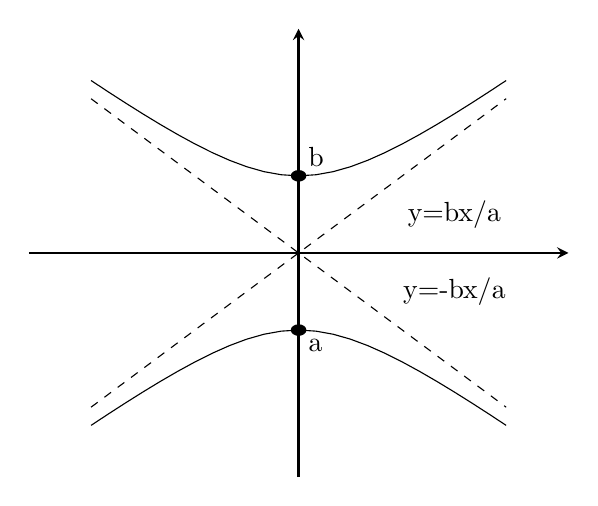
\begin{tikzpicture}
\begin{axis}[standard,domain=-4:4,xtick={\empty},ytick={\empty}]
\addplot[] {(x^2+4)^0.5};
\addplot[] {-(x^2+4)^0.5};
\addplot[dashed] {x};
\fill[] (0,2) circle [radius=0.15] node[above right]{b};
\node[] at (3,1) {y=bx/a};
\addplot[dashed] {-x};
\node[] at (3,-1) {y=-bx/a};
\fill[] (0,-2) circle [radius=0.15] node[below right]{a};
\end{axis}
\end{tikzpicture}
\end{center}

\begin{center}
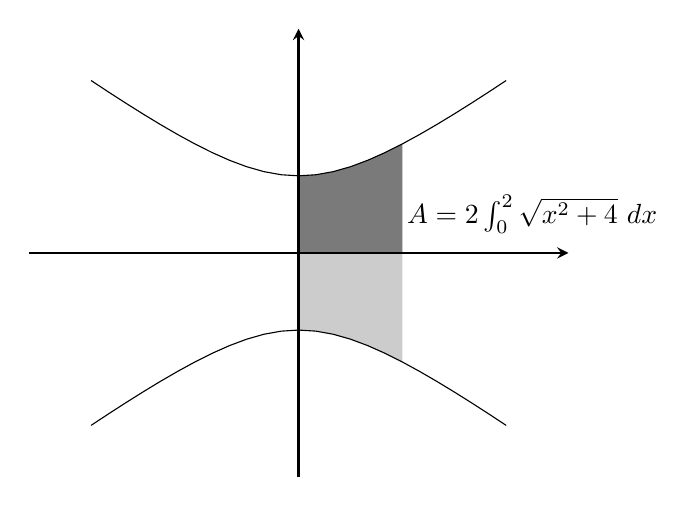
\begin{tikzpicture}
\begin{axis}[standard,domain=-4:4,xtick={\empty},ytick={\empty},clip=false]
\addplot[name path=F] {(x^2+4)^0.5};
\addplot[name path=G] {-(x^2+4)^0.5};
\addplot[name path=H] {0};
\addplot[fill=black, fill opacity=0.2] fill between [of=F and G, soft clip={domain=0:2}];
\addplot[fill=black, fill opacity=0.4] fill between [of=F and H, soft clip={domain=0:2}];
\node[] at (4.5,1) {$A=2\int_0^2\sqrt{x^2+4}\ dx$};

\end{axis}
\end{tikzpicture}
\end{center}

And we could solve this by paramaterizing the equation or using a substitution. Both hyperbolic.

\vspace{10pt}

We are definitely going to be expected to know hyperbolic properties, such as $\sinh2t=2\sinh t\cosh t$. These are similar to their trigonometric counterparts.

\vspace{10pt}

In this class, out problems involved a lot of previous material, such as solving for inverse hyperbolic functions.

\vspace{10pt}

We ended class by studying some volumes.

\begin{center}
\begin{tikzpicture}
\begin{axis}[
standard,
domain=1:4,
xtick={\empty},ytick={\empty},
xmin=0, xmax=5,
ymin=0, ymax=5]
\addplot[]{-0.1*x+0.1*sin(deg(x))+3};
\addplot[]{-0.1*x+0.1*cos(deg(3*x))+2};
\draw[] (1,2.392) circle [y radius=0.592, x radius=0.15];
\draw[] (4,2.104) circle [y radius=0.4203, x radius=0.12];

\draw[very thick] (3,2.1615) circle [x radius=0.13, y radius=0.5525];

\draw[dashed] (1,1.8) -- (1,0) node[pos=1,below]{$a$};
\draw[dashed] (4,1.684) -- (4,0) node[pos=1,below]{$b$};

\fill[] (1,2.984) circle [radius=0.05];
\fill[] (1,1.8) circle [radius=0.05];
\fill[] (4,2.5243) circle [radius=0.05];
\fill[] (4,1.684) circle [radius=0.05];
\end{axis}
\end{tikzpicture}
\end{center}

\[dV=A(x)\ dx;\qquad\int dV=V=\int_a^bA(x)\ dx\]

\vspace{10pt}

{\bf{}EXAMPLE} Volume of conic frustum:

\vspace{10pt}

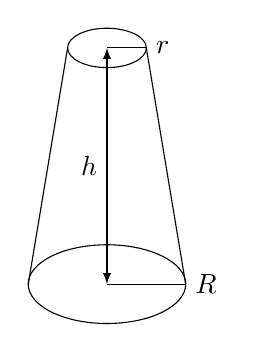
\begin{tikzpicture}
\draw[] (0,0) circle [x radius=1, y radius=0.5];
\draw[] (0,3) circle [x radius=0.5, y radius=0.25];
\draw[latex-latex] (0,0) -- (0,3) node[pos=0.5,left]{$h$};
\draw[] (0,3) -- (0.5,3) node[pos=1,right]{$r$};
\draw[] (0,0) -- (1,0) node[pos=1,right]{$R$};
\draw[] (-1,0) -- (-0.5,3);
\draw[] (1,0) -- (0.5,3);
\end{tikzpicture}
$\Rightarrow$
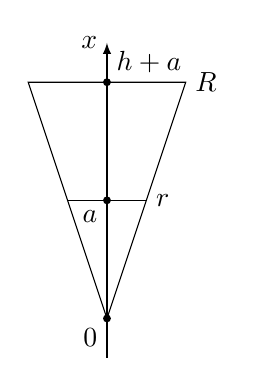
\begin{tikzpicture}
\draw[] (0,0) -- (1,3) -- (-1,3) -- cycle;
\draw[] (-0.5,1.5) -- (0.5,1.5);
\draw[-latex] (0,-0.5) -- (0,3.5);
\fill[] (0,3) circle [radius=0.05] node[above right]{$h+a$};
\fill[] (0,0) circle [radius=0.05] node[below left]{$0$};
\fill[] (0,1.5) circle [radius=0.05] node[below left]{$a$};
\node[right] at (0.5,1.5) {$r$};
\node[right] at (1,3) {$R$};
\node[left] at (0,3.5) {$x$};
\end{tikzpicture}
$\Rightarrow$
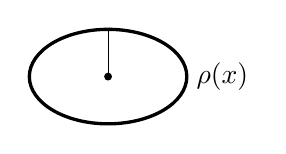
\begin{tikzpicture}
\draw[very thick] (0,0) circle [x radius=1, y radius=0.6];
\fill[] (0,0) circle [radius=0.05];
\draw[] (0,0) -- (0,0.6);
\node[right] at (1,0) {$\rho(x)$};
\end{tikzpicture}




\end{document}

